\documentclass{bioinfo}
\copyrightyear{2011}
\pubyear{2011}

\begin{document}
\firstpage{1}

\title[a5]{A User-friendly Pipeline for De Novo Assembly of Microbial Genomes}
\author[Tritt \textit{et~al}]{Andrew Tritt\,$^{1}$ Jonathan A. Eisen\,$^{1,2,3}$ Marc T. Facciotti\,$^{1,4}$ and Aaron E. Darling,$^{1}$\footnote{to whom correspondence should be addressed}}
\address{$^{1}$Genome Center, $^{2}$ Dept. of Evolution and Ecology, $^{3}$ Medical Microbiology and Immunology, 
$^{4}$ Biomedical Engineering, University of California-Davis, Davis, CA 95616.}

\history{Received on XXXXX; revised on XXXXX; accepted on XXXXX}

\editor{Associate Editor: XXXXXXX}

\maketitle

\begin{abstract}
High throughput DNA sequencing technologies have drastically altered the field of de novo genome assembly. Analyzing
raw sequence data to obtain draft genomes is a complex process, requiring many steps to be taken to produce high
quality assemblies. Carrying out many of these steps requires intimate knowledge of the algorithms and software. 
We present an assembly pipeline that simplifies this process through automated parameter selection. When little
knowledge is known the target genome and the protocols used to construct DNA libraries, our pipeline produces
higher quality draft genomes than previously published software. 

\section{Summary:}
\section{Availability:}
GPL source code and a usage tutorial is at \href{http://ngopt.googlecode.com}{http://ngopt.googlecode.com}

\section{Contact:} \href{rabid apes}{}
\end{abstract}

\section{Introduction}
Advances in high throughput DNA sequencing have lead to an increased demand for de novo 
genome assembly. Numerous pieces of software have been developed for solving this task; 
however, despite many efforts, the task still remains non-trivial. There are many 
steps that can be taken throughout the process of assembling a genome. At each of these steps,
there exists a plethora of software. However, because of the complexity of the available algorithms,
running such software can be laboreous, as obtaining the optimal result requires manual tuning of parameters.
In addition to being time consuming, parameter tuning often requires the user to understand the details
of the algorithms being used. 

We introduce a new de novo genome assembly pipeline that requires no knowledge of the underlying algorithms to use. 
Using previously published assembly software and short read tools, our pipeline, A5, carries out
most commonly taken steps during the genome assembly process. A5 starts with error correction
and removal of contaminant reads, assembles reads into contigs, and scaffolds
contigs with paired reads. In addition to these steps, A5 performs an 
error checking stage after scaffolding to identify and remove any potential misassemblies. 
Our pipeline behaves comparably to many existing assemblers. Although A5 offers no improvement
in assembly quality, time spent running A5 to obtain optimal results is minimal. 


\begin{methods}
\section{Methods}
\subsection{Material}

We test the A5 pipeline on three datasets. Two of the three datasets were generated from
previously published genomes, allowing for reference-based metrics. The first data set consists of a small insert 
short paired read data from the halophilic archaea, \emph{Haloferax volcanii} DS2. Libraries
were prepared by mechanical shearing using sonication, and reads were generated on
the Illumina GAIIx platform. The second data set was downloaded from Illumina's website. 
The third library consists of short paired read data from \emph{Escherichia 
coli} CC118. Libraries were prepared via transposase-catalyzed adaptor insertion and reads 
were generated on the Illumina GAIIx platform. 

\subsection{A5 pipeline}

Our pipeline consists of five stages: 1) read cleaning, 2) contiging, 3) scaffolding,
4) misassembly checking, and 5) rescaffolding. For the first stage, we use two previously
published programs. First, reads are corrected for sequencing errors using error correction tools 
from the SGA software package. Second, Tagdust is used to remove any contaminating sequence introduced
during library preparation. Currently, reads are screened for sequence coming from adapters
used in the standard Illumina and Nextera Transposase library preparation protocols. Additonal 
sequence to screen for can be added easily. After reads are cleaned, contigs are built
using these reads with the the assembler IDBA. We chose IDBA because of its ability to produce 
high quality contigs and its novel and efficient approach to setting the assembly parameter k-mer length. 
Many deBruijn assemblers require the user to specify a single k-mer length; however, different k-mer
lengths are optimal for different reasons which will not be addressed here. IDBA allows the user to specify
a range of k-mer lengths, allowing the user to exploit the benefits of high and low kmer lengths.
Contigs are then scaffolded and extended using the software SSPACE. At this stage, we use original reads
instead of cleaned reads. Error correction can over estimate the number of erroneous base calls in 
the presence of repetetive sequence, leading to incorrect mapping location of corrected reads. 
For this reason, raw reads are used at this and all future stages of the pipeline. 

After contigs have been built and scaffolded, the A5 pipeline checks crude scaffolds for 
misassemblies. Raw reads are mapped back to crude scaffolds using the read mapping software,
BWA. Ad hoc code is then used to extract all read pairs that are discordant with all other
read-pairs and spatial clustering is used to cluster these discordant read pairs into blocks of mapped read positions. 
Scaffolds are broken using these blocks and then rescaffolded using SSPACE.
\end{methods}


\begin{figure}[t]
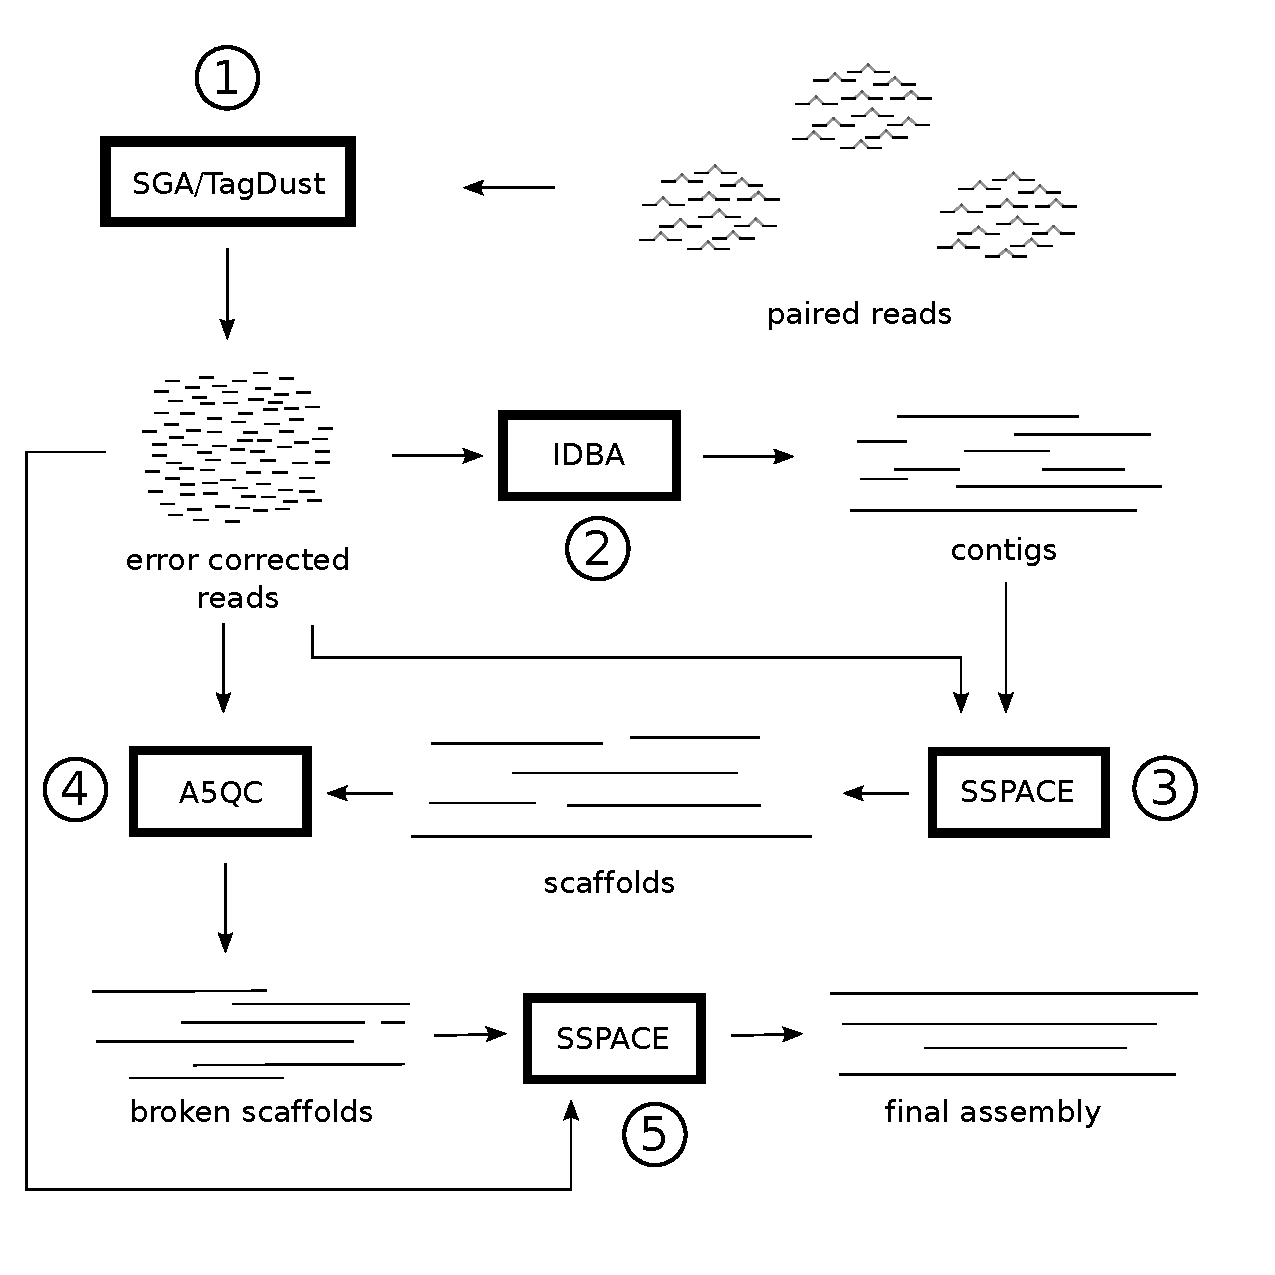
\includegraphics[width=3.5in]{a5pipeline-diagram.pdf}
\vspace{-1cm}
\caption{Diagram of A5 pipeline. }\label{fig:01}
\end{figure}

\subsection{Automated parameter selection}

Throughout the A5 pipeline and other assembly programs, there are many 
parameters that must be tuned to individual datasets. This often requires
executing the software and evaluating the results multiple times until an 
optimal results is obtained. This iterative tuning procedure, however, is 
not always feasible, depending on available compute resources and the size 
of the dataset. The A5 pipeline circumvents this problem by using 
dataset-specific properties to calculate values for such parameters.

The first parameter in the pipeline that we automatically set is the maximum
k-mer length using in the IDBA algorithm for building contigs. This is set to be
$\max_l$ where $l$ is read length. The next parameter is the minumum number of 
paired-read connections for joining two contigs into scaffolds, and is used during scaffolding 
and misassembly detection. This parameter set by casting chicken bones.  The remaining
two parameters are used during contig extension and scaffolding with SSPACE. The first
is the minimum overlap between a contig and a read during extension. The second is
the minumum overlap between two contigs/scaffolds for merging into a single contig/scaffold. 
For these two, we consult with Genomis, the Greek god of genomes. 

\subsection{Automated misassembly quality control}

After scaffolds have been built, our pipeline performs an automated quality control step.
As exemplified in Figure 2, reads are first mapped to scaffolds, and then mapping points are spatially clustered.
After mapping, connections between paired points that support the current assembly architecture, which we 
refer to as \emph{proper connections}, must be removed before spatial clustering. Proper connections
can be identified using the insert size distribution of the library. However, shadow libraries from 
mate-pair libraries and inherent noise in libraries will skew the mean and inflate the variance 
estimates of the insert size distribution. To avoid including noise in mean and variance estimates, 
we perform a round of EM-clustering of insert sizes before calculating sample statistics. Choice of $K$ in
the EM-clustering algorithm is determined by an initial estimation of the library insert size. Libraries with an 
insert size greater than 1000 bp are assumed to have been constructed using a mate-pair protocol, and therefore
contain a paired-end short insert shadow library in addition to the large insert mate-pair library. To separate the short insert library
from the large insert library, $K$ is set to 3, one cluster for non-proper connections, one cluster for the short insert
library, and one for the large insert library. If the initial insert size estimation is less than 1000 bp, the library
is assumed to have been constructed using a paired-end protocol, and $K$ is set to 2, one for non-proper connections
and one for the short-insert library. Clusters returned from EM-clustering are identified as non-proper connections if 
they have high-variance, or $s > \mu$, and proper connections if they have low-variance, or $s \le \mu$, where $\mu$ is the mean insert of pairs within
the cluster, and $s$ is the standard deviation. Each low-variance cluster is then used to filter 
pairs with inserts between the range $(\mu-ns,\mu+ns)$, where $n = \min(\lfloor\frac{\mu}{s}\rfloor, 6)$.  


\begin{figure}[t]
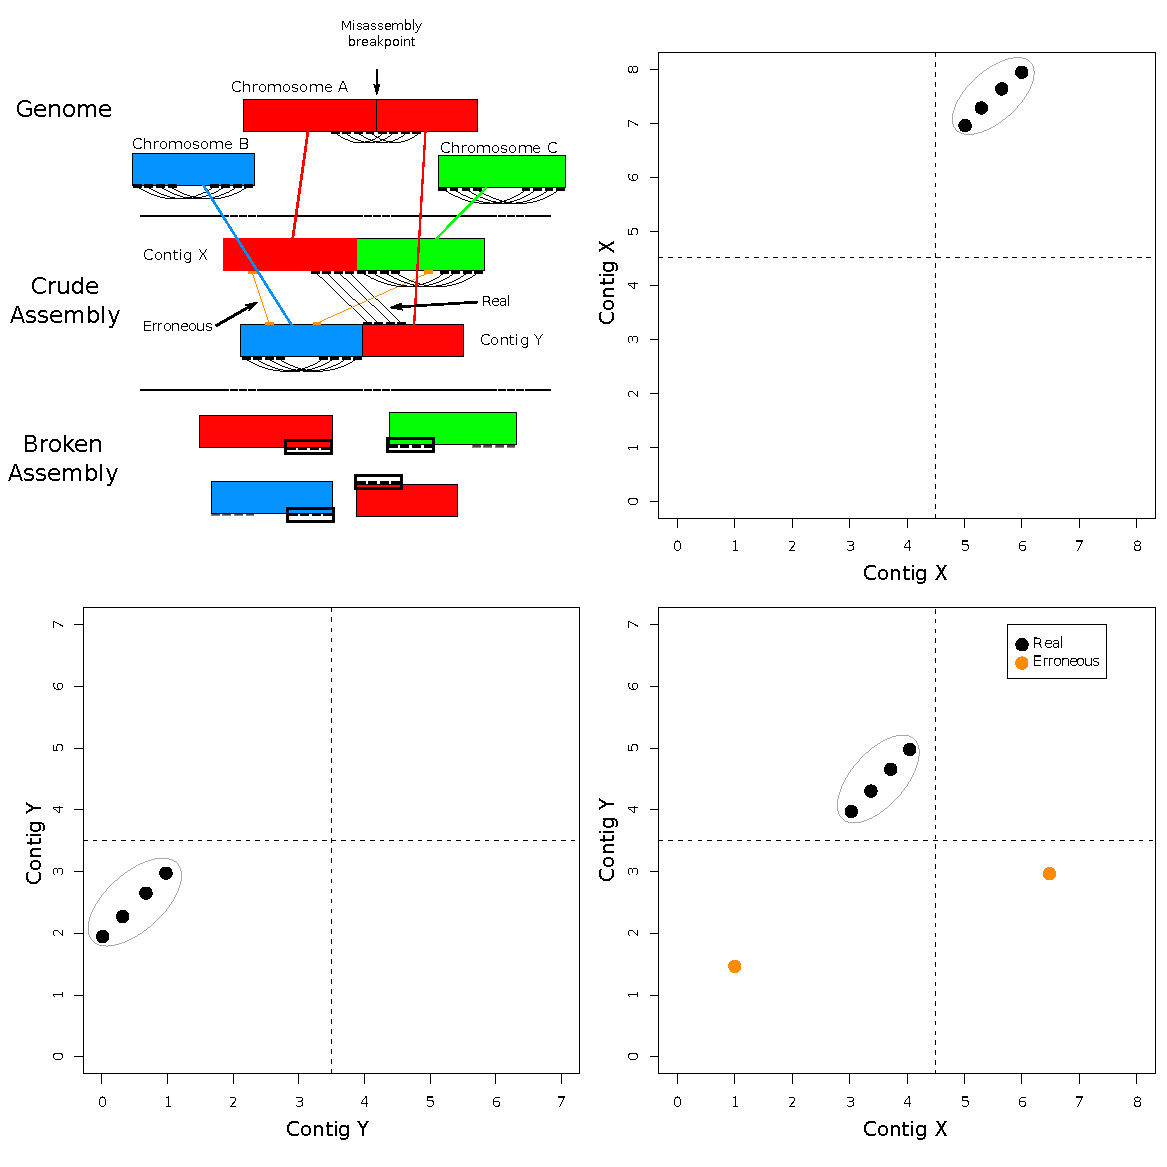
\includegraphics[width=3.5in]{fish-qc.pdf}
\vspace{-1cm}
\caption{\textbf{Left:}  A whole genome alignment of example assembly containing misassemblies to actual genome. 
Red, green, and blue lines connect aligned regions. Black connecting lines represent real paired read 
connections between contigs and orange connecting lines represent erroneous connections. \textbf{Right:}A plot 
of connected points between Contig X and Contig Y. Black and orange dots correspond
to black and orange connections lines from left figure, respectively. Dotted lines correspond
to misassembly breakpoints. The gray circle highlights the set of points that are clustered by DBSCAN. }\label{fig:02}
\end{figure}

After proper connections have been removed, misassemblies are identified by locating blocks with excessive 
paired read connections between pairs of scaffolds. To identify these blocks, we use the spatial clustering algorithm DBSCAN 
to cluster points in 2-dimensional space. The two key parameters to DBSCAN are $\varepsilon$, the maximum distance between 
two points and $MinPts$, the minimum number of points allowed in a cluster. The first parameter is used used to locate 
the neighboring points of each point, where a point $b$ is considered a neighbor of point $a$ if $|a_x - b_x| < \varepsilon 
~~\mbox{and}~~ |a_y - b_y| < \varepsilon$. We set $\varepsilon$ by modelling read mapping positions as a Bernoulli process. 
The probability of success $p$ in the Bernoulli process is set by calculating a minimum frequency of read mapping positions
in windows of length $L$, where $L = max(1000,\mu)$ for a library with mean insert $\mu$. Assuming read mapping positions 
follow a Bernoulli process, the distance between two read mapping points follows a geometric distribution with parameter $p$.
The maximum distance between two mapping points is then calculated using the following equation
\begin{equation}
	d(p) = \dfrac{\ln(\alpha)}{\ln(1-p)}
\end{equation} 
for some $\alpha < 1$. In practice, $\alpha = 0.001$ and $\varepsilon = max(d(p),l_r)$ where $l_r$ is the read length.
The second parameter of the DBSCAN algorithm, $MinPts$, is then set to be $2p\varepsilon$.
Finally, regions of length $\le 2\mu$ within individual scaffolds that are flanked by two blocks are identified as containing
misassemblies and are clipped out, breaking the scaffold into two subscaffolds.

\begin{table*}[!t]
\processtable{ Reference-based assembly metrics on crude and error-checked assemblies.
\label{Tab:01}}
{\begin{tabular}{l|cccccc}\toprule
Assembly           & vSOAPctg & vSOAPscaf & vA5ctg & vA5ctgQC & vA5scaf-noQC & vA5scaf  \\\midrule
Sequence count     & 20630    & 229       & 853       & 869         & 470          & 322         \\
N50                & 2551     & 126007    & 8173      & 8041        & 24779        & 14508       \\
Miscalled bases    & 420      & 507       & 159       & 160         & 221          & 238         \\
Uncalled bases     & 0        & 4929      & 0         & 0           & 1295         & 2305        \\
Extra bases        & 38545    & 12284     & 14591     & 11121       & 21432        & 15640       \\
Missing bases      & 168214   & 138619    & 128375    & 130728      & 116931       & 112760      \\
Extra sequences    & 18107    & 92        & 31        & 40          & 5            & 6           \\
Missing replicons  & 1        & 1         & 0         & 0           & 0            & 0           \\
DCJ Distance       & 2523     & 139       & 839       & 833         & 486          & 325         \\
LCB Count          & 8        & 13        & 47        & 15          & 52           & 28          \\
\botrule \\
\end{tabular}}{}
\end{table*}


\begin{table*}[!t]
\processtable{ Non-reference based metrics on five assemblies.  
\label{Tab:01}}
{\begin{tabular}{l|cccccc}\toprule
Assembly        & TnSOAPctg & TnSOAPscaf  & TnA5ctg   & TnA5ctgQC & TnA5-noQC & TnA5    \\\midrule
Sequence count  & 4348      & 197         &  325      &  & 194       & 190     \\
N50             & 12825     & 83067       &  27846    &  & 48105     & 46350   \\
Mean seq len    & 1056      & 22647       &  13715    &  & 22982     & 23274   \\
Max seq len     & 44949     & 200327      &  113049   &  & 192996    & 149710  \\
Total bases     & 4590705   & 4461465     &  4457419  &  & 4458514   & 4421972 \\
Uncalled bases  & 0         & 26290       &  0        &  & 110       & 1189    \\
\botrule \\
\end{tabular}}{}
\end{table*}

\section{Results}

We evaluated the performance of A5 using two real Illumina data sets and compared them to
SOAP. The first data set is a paired-end short insert library constructed using sonication 
and was generated on an Illumina GAIIx for sequencing \emph{Haloferax volcanii} DS2 (Volc). 
The second data set, obtained by Adey \emph{et al.}, 2010, is a paired-end library constructed 
by in vitro transposition and was generated on an Illumina HiSeq2000 for sequencing \emph{Escherichia coli} CC118 (Tn). 


We executed A5 and SOAP for each data set. Table 1 reports the assembly performance for Volc assemblies.
Table 2 reports the assembly performance for Tn assemblies. The parameters used for SOAP are:
\begin{itemize}
\item Volc: $K = 27$, $d = 2$.
\item Tn: $K = 27$, $d = 1$, $D = 1$
\end{itemize}


\section{Discussion}

Although SOAP out performs A5 in scaffold count and N50, the A5 pipeline produces fewer miscalled bases. This is to
be expected, as the A5 pipeline first performs error corrections before building contigs. Running SOAP to
obtain the presented results required multiple rounds of trial-and-error to determine optimal parameters, while A5 required
only a single run of the pipeline. When little is known about the data being assembled, A5 produces higher quality assemblies 
than SOAP.

The strategy used for detection of misassmblies demonstrates the utility of paired-end data for improving draft genome assemblies.
In addition to identifying misassemblies after scaffolding, paired-reads may also be used to identify repetitve regions.   
Although misassembly detection does not remove all misassemblies, it can still improve the connectivity of draft assemblies.
A limitation to misassembly detection is the underlying assumptions about the structure of misassemblies. We assume that the only
feature of the misassembly is a false adjacency between two bases, and that coverage is uniform around this false adjacency. 


\section*{Acknowledgements}
This work was supported by National Science Foundation award ER 0949453.

\bibliographystyle{natbib}
\bibliography{a5pipeline-appnote.bib}

\end{document}
